\appendix

\renewcommand{\theequation}{\Alph{chapter}-\arabic{equation}}
\renewcommand{\thefigure}{\Alph{chapter}-\arabic{figure}}

\chapter{Heat transfer under constant temperature}
\label{cha:CTHX}
Assuming $U$, $T_{c}$, $\dot{m}$, $c_{p}$ to be constant, for given $T_{i}$,

\begin{figure}[h]
\centering
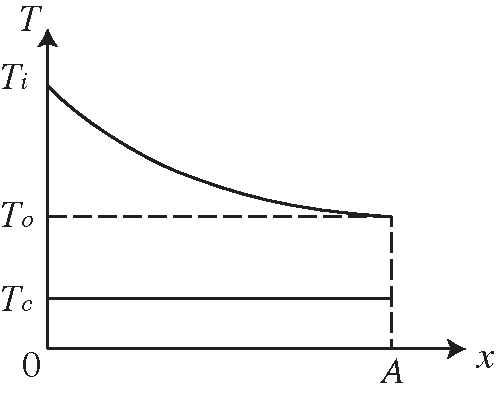
\includegraphics[width=0.6\textwidth]{fig/ConstTempHX.pdf}
\caption{Diagram of heat transfer under constant temperature}
\label{fig:CTHX}
\end{figure}
 
Set $x$ as the area involved in the transfer heat process, when $x$ from $0$ to $A$, $T(x)$ from $T_{i}$ to $T_{o}$,
\begin{equation}
\dot{m}c_{p}dT(x)=(T_{c}-T(x))Udx
\end{equation}
so
\begin{equation}
\frac{dT(x)}{dx}=-\frac{U}{\dot{m}c_{p}}(T(x)-T_{c})
\end{equation}
\begin{equation}
T_{g}(x)=T_{p}(x)+T_{h}(x)
\end{equation}
where $T_{g}(x)$ is the general solution, $T_{p}(x)$ is the particular
solution, $T_{h}(x)$ is the homogeneous solution.

\begin{equation}
-\frac{U}{\dot{m}c_{p}}(T_{p}(x)-T_{c})=0
\end{equation}
\begin{equation}
T_{p}(x)=T_{c}
\end{equation}
\begin{equation}
\frac{dT_{h}(x)}{dx}=-\frac{U}{\dot{m}c_{p}}T_{h}(x)
\label{eq:T_h(x)}
\end{equation}

\begin{equation}
\int_{T_{h}(x)=T_{h}(0)}^{T_{h}(x)=T_{h}(A)}\frac{dT_{h}(x)}{T_{h}(x)}=-\int_{x=0}^{x=A}\frac{U}{\dot{m}c_{p}}dx
\end{equation}
\begin{equation}
\frac{T_{h}(A)}{T_{h}(0)}=\exp(-\frac{UA}{\dot{m}c_{p}})
\end{equation}
that is
\begin{equation}
\frac{T_{g}(A)-T_{p}(A)}{T_{g}(0)-T_{p}(0)}=\exp(-\frac{UA}{\dot{m}c_{p}})
\end{equation}
\begin{equation}
\frac{T_{o}-T_{c}}{T_{i}-T_{c}}=\exp(-\frac{UA}{\dot{m}c_{p}})
\label{eq:Eq}
\end{equation}

\chapter{Thermal gradient under constant heat flux}\label{cha:CTCHFHX}

Assuming $U$, $T_{c}$, $\dot{m}$, $c_p$, $q''$ to be constant, for
given $T_{i}$,
\begin{figure}[h]
\centering
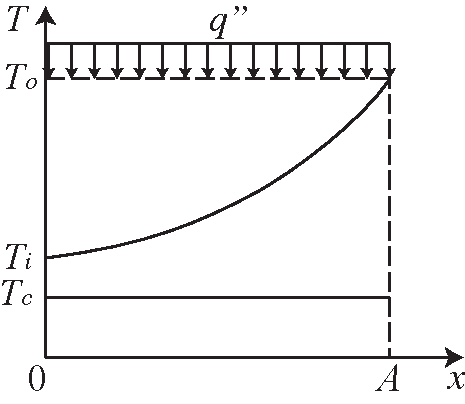
\includegraphics[width=0.6\textwidth]{fig/CTCHFHX.pdf}\caption{Diagram of heat transfer with one constant temperature
heat source and constant heat flux}
\label{fig:CTCHFHX}
\end{figure}

Set $x$ as the area involved in the transfer heat process, when $x$ from $0$ to $A$, $T(x)$ from $T_{i}$ to $T_{o}$,
\begin{equation}
\dot{m}c_{p}dT(x)=(T_{c}-T(x))Udx+q''dx
\end{equation}
so
\begin{equation}
\frac{dT(x)}{dx}=-\frac{UP}{\dot{m}c_{p}}T(x)+\frac{q''P+UPT_{c}}{\dot{m}c_{p}}
\end{equation}
\begin{equation}
T_{g}(x)=T_{p}(x)+T_{h}(x)
\end{equation}
where $T_{g}(x)$ is the general solution, $T_{p}(x)$ is the particular
solution, $T_{h}(x)$ is the homogeneous solution.

\begin{equation}
-\frac{U}{\dot{m}c_{p}}T_{p}(x)+\frac{q''+UT_{c}}{\dot{m}c_{p}}=0
\end{equation}
\begin{equation}
T_{p}(x)=T_{c}+\frac{q''}{U}
\end{equation}
\begin{equation}
\frac{dT_{h}(x)}{dx}=-\frac{U}{\dot{m}c_{p}}T_{h}(x)
\end{equation}

It is the same as \autoref{eq:T_h(x)}, so we have
\begin{equation}
\frac{T_{g}(A)-T_{p}(A)}{T_{g}(0)-T_{p}(0)}=\exp(-\frac{UA}{\dot{m}c_{p}})
\end{equation}
\begin{equation}
\frac{T_{o}-T_{c}-\dfrac{q''}{U}}{T_{i}-T_{c}-\dfrac{q''}{U}}=\exp(-\frac{UA}{\dot{m}c_{p}})
\end{equation}

\chapter{MATLAB code of class Stream}
\label{cha:MATLAB_SOURCECODE}

%\begin{lstlisting}[language= MATLAB, backgroundcolor = \color{yellow!20}, title = {The MATLAB source code of the definition of the class -- Stream}, label = {lst:MATLAB_SOURCECODE}]
\begin{lstlisting}[language= MATLAB, backgroundcolor = \color{yellow!20}, label = {lst:MATLAB_SOURCECODE}]
classdef Stream < handle
    %Stream This class describes a fluid stream that has inherent
    %properties and dependent properties
    
    properties
        fluid;  % Fluid type
        dot_m;  % Mass flow rate, kg/s
        T;      % Temperature, K
        p;      % Pressure, Pa
        x;      % Quality, [0, 1] for two phase stream; NaN for single 
                %   phase stream
    end
    properties(Dependent)
        h;      % Mass specific enthalpy, J.kg
        s;      % Mass specific entropy, J/kg-K
        cp;     % Specific heat under constant pressure, J/kg-K
    end
    
    methods
        function obj = Stream
            obj.T = Temperature;
            obj.dot_m = Massflow;
            obj.p = Pressure;
        end
        function flowTo(obj, st)
            st.fluid = obj.fluid;
            st.dot_m = obj.dot_m;
        end
        function st2 = mix(obj, st1)
            % Get the properties of a stream mixed by two streams
            % The two streams must have the same fluid type and pressure
            if obj.fluid == st1.fluid
                if  obj.p.v == st1.p.v
                    obj.p = st1.p;
                    st2.fluid = obj.fluid;
                    st2.p = obj.p;
                    st2.dot_m.v = obj.dot_m.v + st1.dot_m.v;
                    h = (obj.dot_m.v .* obj.h + st1.dot_m.v .* st1.h)...
                        ./ (obj.dot_m.v + st1.dot_m.v);
                    st2.T.v = CoolProp.PropsSI('T', 'H', h, 'P',st2.p.v);
                else
                    error('The two streams have different pressures!');
                end
            else
                error('The two streams have different fluid types!');
            end
        end
        function convergeTo(obj, st, y)
            % Get another stream converged (or diverged)
            % from the original stream state.
            % If y < 1, the original stream is diverged
            % If y > 1, the original stream is converged
            st.fluid = obj.fluid;
            st.T = obj.T;
            st.p = obj.p;
            st.x = obj.x;
            st.dot_m.v = obj.dot_m.v .* y;
        end
    end
    methods
        % The dependent properties can be obtained from the inherent
        %   properties
        % If x is NaN, then the dependent properties are determined
        %   by T and P; otherwise, they are determined by P and x
        function value = get.h(obj)
            if isempty(obj.x)
                value = CoolProp.PropsSI('H', 'T', obj.T.v, ...
                    'P', obj.p.v, obj.fluid);
            else
                value = CoolProp.PropsSI('H', 'P', obj.p.v, 'Q', ...
                    obj.x, obj.fluid);
            end
        end
        function value = get.s(obj)
            if isempty(obj.x)
                value = CoolProp.PropsSI('S', 'T', obj.T.v, ...
                    'P', obj.p.v, obj.fluid);
            else
                value = CoolProp.PropsSI('S', 'P', obj.p.v, 'Q', ...
                    obj.x, obj.fluid);
            end
        end
        function value = get.cp(obj)
            if isempty(obj.x)
                value = CoolProp.PropsSI('C', 'T', obj.T.v, ...
                    'P', obj.p.v, obj.fluid);
            else
                value = inf;
            end
        end
    end
end
\end{lstlisting}
  
\begin{publications}
  \item Cheng Zhang, Yanping Zhang, Inmaculada Arauzo, Wei Gao, Chongzhe  Zou. Cascade system using both trough system and dish system for power generation. Energy Conversion and Management. 2017.06.15;142:494–503.
  \item Cheng Zhang, Yanping Zhang, Xiaolin Lei, Wei Gao. Design and Comparison of Solar Thermal Oilfield Steam Production System Plans. Journal of Solar Energy Engineering. 2017.01.08;139;004502-4.
  \item Cheng Zhang, Kun Wang, Jizhou Wang, Shuhong Huang. FEA simulation on the alignment of the shafts of three-fulcrum turbine. International Conference on Power Engineering. 2013.
  \item Chongzhe Zou, Yanping Zhang, Quentin Falcoz, Pierre Neveu, Cheng Zhang, Shuhong Huang, Weicheng Shu. Design and Optimization of a High-temperature Cavity Receiver for a Solar Energy Cascade Utilization System. Renewable Energy. 2017.04.01:103; 478-89. 
  \item Chongzhe Zou, Yanping Zhang, Huayi Feng, Quentin Falcoz, Pierre Neveu, Cheng Zhang, Wei Gao. “Effects of Geometrical Parameters on Thermal Performance for a Cylindrical Solar Receiver Using 3D numerical Model.” Energy Conversion and Management, 2017.10.1: 126-17.
  \item Chongzhe Zou, Yanping Zhang, Quentin Falcoz, Pierre Neveu,Cheng Zhang. Thermal modeling of a pressurized air cavity receiver for solar dish Stirling system, Solarpaces: International Conference on Concentrating Solar Power \& Chemical Energy Systems. AIP Publishing LLC, 2017:1884-1892.
  
  \item A solar thermal cascade system, No. 201610806296.5
  \item A flow control method used in a multistage heating system, No. 201610805604.2
  \item Software copyright registration: solar thermal power development system (registration number: 2017SR382378), authorization date: 2017.7.19
  
\end{publications}

\nomenclature[S]{$i$}{Inlet}
\nomenclature[S]{$g$}{General solution}
\nomenclature[S]{$o$}{Outlet}